
\documentclass[xcolor={usenames,dvipsnames},12pt,presentation,aspectratio=169]{beamer}

\usepackage[utf8]{inputenc}
\usepackage{fontawesome}
\usepackage[brazilian]{babel}
\usepackage{verbatim}
\usepackage{graphicx}
\usepackage{xspace}
\usepackage{amsthm}
\usepackage{url}
\usepackage{array}
\usepackage{hyperref}
\usepackage{times,mathptmx}
\usepackage{pdfpages}
\usepackage{mdframed}
\usepackage{tikz}
\usepackage{alltt}
\usepackage{minted}
%\usepackage{times}
%\usepackage[usenames,dvipsnames]{xcolor}
%\usepackage[usenames,dvipsnames]{color}
%\usepackage{color}

\usetikzlibrary{arrows,shapes}

\usetheme{Madrid}
%\usetheme{Boadilla}
%\usetheme{Darmstadt}
%\usetheme{Frankfurt}
%\usetheme{CambridgeUS}
%\usetheme{AnnArbor}
%\usecolortheme{beaver}
%\usecolortheme{seahorse}
%\usecolortheme{seagull}
\usecolortheme[named=BrickRed]{structure}

\setbeamercovered{transparent}

\setbeamertemplate{footline}[frame number]
%\setbeamertemplate{navigation symbols}{}
%\setbeamersize{text margin left=1em,text margin right=1em}

\newcommand{\titulo}{Programação Paralela com OpenMP}
\newcommand{\disciplina}{ELC139 - Programação Paralela}
\newcommand{\nome}{João Vicente Ferreira Lima (UFSM)}

\lecture[1]{\aula}{aula01}
\def\lecturename{\aula}

\newcommand{\Red}[1]{{\color{red}#1}}
\newcommand{\red}[1]{{\color{red}#1}}
\newcommand{\Blue}[1]{{\color{blue}#1}}
\newcommand{\blue}[1]{{\color{blue}#1}}

\newcommand{\PBS}[1]{\let\temp=\\#1\let\\=\temp}
\newcommand{\RRCOL}{\PBS\raggedright\hspace{0pt}}

\newcommand{\p}[1]{\texttt{#1}}
\newenvironment{code}{%
  \begin{alltt}%
  }{%
  \end{alltt}%
}

% https://github.com/joao-lima/ATPESC

\makeatletter
%\setbeamertemplate{headline}{}
% {%
%   \leavevmode%
%   \@tempdimb=2.4375ex%
%   \ifnum\beamer@subsectionmax<\beamer@sectionmax%
%     \multiply\@tempdimb by 4%
%   \else%
%     \multiply\@tempdimb by\beamer@subsectionmax%
%   \fi%
%   \ifdim\@tempdimb>0pt%
%     \advance\@tempdimb by 1.125ex%
%     \begin{beamercolorbox}[wd=.5\paperwidth,ht=\@tempdimb]{section in head/foot}%
%       \vbox to\@tempdimb{\vfil\insertsectionnavigation{.5\paperwidth}\vfil}%
%     \end{beamercolorbox}%
%     \begin{beamercolorbox}[wd=.45\paperwidth,ht=\@tempdimb]{subsection in head/foot}%
%       \vbox
%       to\@tempdimb{\vfil\insertsubsectionnavigation{.45\paperwidth}\vfil}%
%     \end{beamercolorbox}%
%     \begin{beamercolorbox}[wd=.05\paperwidth,ht=\@tempdimb]{subsection in head/foot}%
%       \vbox
%       to\@tempdimb{\vfil\hfil\insertframenumber\vfil\vfil}%
%     \end{beamercolorbox}%
%   \fi%
% }

\def\dohead{\beamer@headcounter=4\relax\beamer@headcounter=1\loop\ifnum\beamer@headcounter<\beamer@totalheads%
  \advance\beamer@headcounter by1\relax%
  \csname @@head\the\beamer@headcounter\endcsname\repeat}

\makeatother

\title[\titulo]{\titulo}

\subtitle{\disciplina}

\author[João V. F. Lima]{\nome}

%\institute[UFSM]{Departamento de Linguagens e Sistemas de Computação \\ Universidade Federal de Santa Maria \\ \url{jvlima@inf.ufsm.br} \\ \url{http://www.inf.ufsm.br/~jvlima}}
\institute[UFSM]{Universidade Federal de Santa Maria \\ \url{jvlima@inf.ufsm.br} \\ \url{http://www.inf.ufsm.br/~jvlima}}
\date{2023/1}

\graphicspath{{.}{figs/}}

\logo{ 
\includegraphics[height=1.5cm,width=1.5cm,keepaspectratio]{logo_inf}    
        
\includegraphics[height=1.5cm,width=1.5cm,keepaspectratio]{logo_ufsm} }

%\titlegraphic{
%	
\includegraphics[width=2cm]{logo_ufsm}
%  \hspace{1cm}
%	
\includegraphics[width=2cm]{logo_inf}
%}

\newtheorem{mydef}{Definição}[section]
%\newtheorem{myteo}{Teorema}[section]
%------------------------------------------------------------------------------
%\newcommand{\xkaapi}{XKaapi\xspace}
%------------------------------------------------------------------------------
% Typesetting Listings
\usepackage{listings}
\lstset{
  language=C,
  %basicstyle=\scriptsize\ttfamily,
  %basicstyle=\normalsize\ttfamily,
  basicstyle=\small\ttfamily,
  %basicstyle=\footnotesize\ttfamily,
  %aboveskip=0pt,
  %belowskip=0pt,
  %mathescape=false,
  columns=fullflexible,
  %numbers=none,
  numbers=left,
  numbersep=5pt,
%  showtabs=true,
%  showspaces=true,
  frame=tb,
  breaklines=true
}
%------------------------------------------------------------------------------
%\lstset{commentstyle=\color{blue}}
%\lstset{stringstyle=\ttfamily}
%\lstset{ classoffset=1, 
%            morekeywords={kaapi,omp,task,data,alloca, declare, reduction, identity, parallel,sync,taskwait,cilk,spawn,tbb,css,cilk\_spawn,cilk\_sync,cilk\_for,offload},
%            keywordstyle=\color{Red}\bfseries
%           }
%\lstset{ classoffset=2, 
%            morekeywords={value,read,write,readwrite,reduction,untied,firstprivate,TaskBodyCPU,TaskBodyGPU,ka,Signature,RW,CW,range2d\_r,range2d\_rw,range2d,Spawn,Fork,Shared\_w,Shared\_r,Shared,a1,target,device,copyin,copyout,input,implements,copy\_deps,RPWP,range2d\_rpwp,rangeindex,Memory,Register,SetStaticSched,Sync,Unregister,Community,System,join\_community,SpawnMain,leave,initialize,terminate,logfile,array,SetArch,ArchHost,ArchCUDA,W,R,gpuStream,pointer\_w,pointer\_r,pointer\_cw,pointer},
%            keywordstyle=\color{Blue}\bfseries
%           }
%\lstset{ classoffset=3, 
%            morekeywords={storage,ld},
%            keywordstyle=\bfseries
%           }
%\lstset{ classoffset=4, 
%            morekeywords={in,out,inout,cout,concurrent},
%            keywordstyle=\color{Red}\bfseries
%           }
%           
%\lstset{classoffset=0, showstringspaces=false}
%------------------------------------------------------------------------------
\mdfsetup{
  backgroundcolor=gray!10,
%  roundcorner=10pt,
}
%------------------------------------------------------------------------------
\newcommand{\restorefootline}{\setbeamertemplate{navigation symbols}{}}
%\newcommand{\setfootline}[1]{\setbeamertemplate{navigation symbols}{\textcolor{black}{\textbf{#1}}}}
\newcommand{\includeslides}[4]{%
%  \setfootline{#1}%
  {
    \setbeamercolor{background canvas}{bg=}
    \includepdf[pages={#1},%
    pagecommand={},
%    pagecommand={\begin{frame}[default]{}\end{frame}},
%    #4,%
    turn=false,noautoscale=false,column=false,columnstrict=false,openright=false,frame=false]{#2}%
  }
  %\restorefootline%
}
%------------------------------------------------------------------------------
\begin{document}

\begin{frame}
%  \titlepage
  \maketitle
%  \mode<presentation>
%  {
%    \begin{columns}
%      \begin{column}{0.5\textwidth}
%      \raggedleft
%	
\includegraphics[width=2cm]{logo_ufsm}
%      \end{column}
%      \begin{column}{0.5\textwidth}
%	
\includegraphics[width=2cm]{logo_inf}
%      \end{column}
%    \end{columns}
%  }
\end{frame}

\begin{frame}
    \frametitle{Outline}
%    \tableofcontents[hideallsubsections]
    \tableofcontents
\end{frame}

\AtBeginSection{
  \begin{frame}
    \frametitle{Outline}
    \tableofcontents[currentsection]
  \end{frame}
}

\AtBeginSubsection[]
{
    \begin{frame}
        \frametitle{Outline}
        \tableofcontents[currentsection,currentsubsection]
    \end{frame}
}

%\begin{minted}[linenos, fontsize=\small, breaklines=true, frame=lines]{C}
%\end{minted}

%%%%%%%%%%%%%%%%%%%%%%%%%%%%%%%%%%%%%%%%%%%%%%%%%%%%%%%%%%%%%%%%%%%%%%%%%%%%%%%
\section{Introdução}
%%%%%%%%%%%%%%%%%%%%%%%%%%%%%%%%%%%%%%%%%%%%%%%%%%%%%%%%%%%%%%%%%%%%%%%%%%%%%%%
\begin{frame}[fragile]
  \frametitle{Programação em OpenMP}
  \begin{itemize}
  \item Epecificação de uma API para paralelismo em \blue{memória compartilhada}
  \end{itemize}
  \begin{center}
    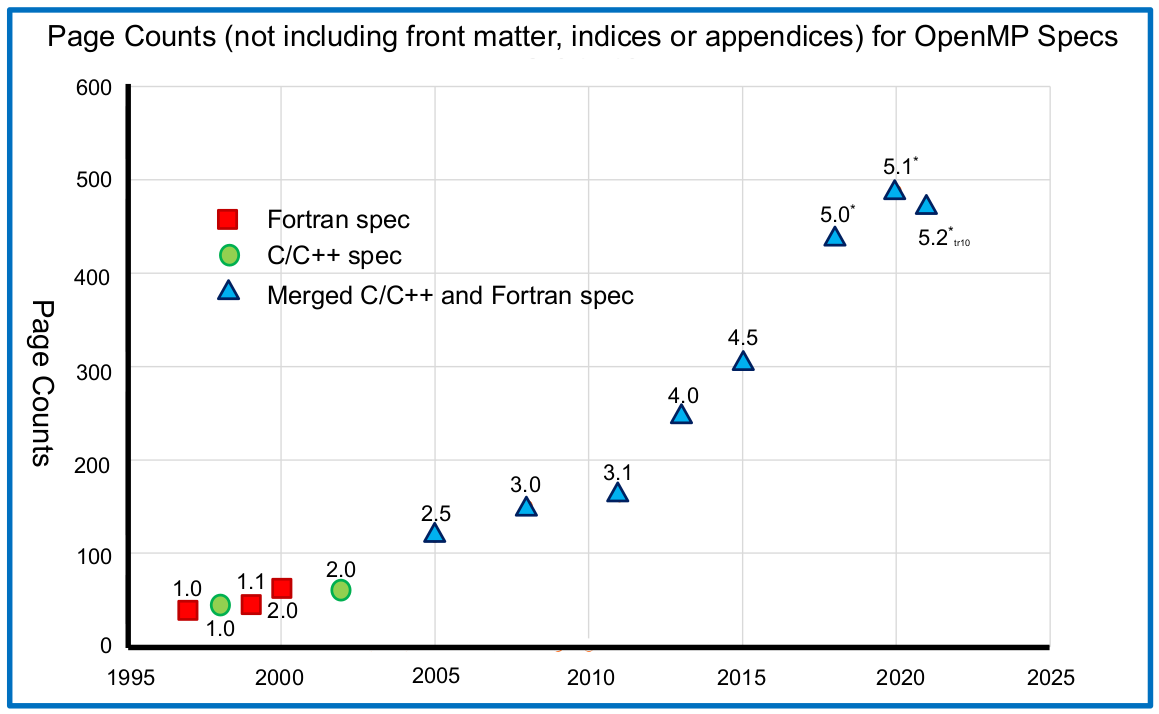
\includegraphics[width=0.6\textwidth]{timespec.png}
   \end{center}  
  \vspace{-4mm}
  {\tiny An Introduction to Parallel programming with OpenMP, Tim Mattson, 2022.}  
\end{frame}
%%%%%%%%%%%%%%%%%%%%%%%%%%%%%%%%%%%%%%%%%%%%%%%%%%%%%%%%%%%%%%%%%%%%%%%%%%%%%%%
\begin{frame}[fragile]
  \frametitle{Programação em OpenMP}
  \begin{itemize}
  \item Paralelismo em \blue{memória compartilhada}
  \item API construída sobre
    \begin{itemize}
    \item {\bf Diretivas de compilação}
    \item Métodos de biblioteca
    \item Variáveis de ambiente
    \end{itemize}
  \end{itemize}
  %
  \onslide<2->
  %
  \begin{itemize}
    \item As diretivas possuem {\bf construções} e {\bf cláusulas}
      \begin{itemize}
      \item {\bf Construções} - seções paralelas, divisão de dados ou tarefas, sincronização
      \item {\bf Cláusulas} - modificam ou especificam aspectos de construções
      \end{itemize}
    \end{itemize}  
  %
  \onslide<3->
  %
  \begin{minipage}{0.95\textwidth}  
    \begin{minted}[linenos, fontsize=\small, breaklines=true, frame=lines]{C}
#pragma omp
\end{minted}
\end{minipage}

\end{frame}
%%%%%%%%%%%%%%%%%%%%%%%%%%%%%%%%%%%%%%%%%%%%%%%%%%%%%%%%%%%%%%%%%%%%%%%%%%%%%%%
\begin{frame}[fragile]
  \frametitle{Hello World!}
  A construção \texttt{parallel} executa o {\bf bloco estruturado} em paralelo.
  %
\begin{minipage}{0.95\textwidth}  
\begin{minted}[linenos, fontsize=\small, breaklines=true, frame=lines]{C}
#include <omp.h>
int main(void) {
  #pragma omp parallel
  {
    int id = omp_get_thread_num();
    int nthreads = omp_get_num_threads();
    printf("Hello world from thread %d of %d\n", id, nthreads);
  }
}
\end{minted}
\end{minipage}
\end{frame}
%%%%%%%%%%%%%%%%%%%%%%%%%%%%%%%%%%%%%%%%%%%%%%%%%%%%%%%%%%%%%%%%%%%%%%%%%%%%%%%
\begin{frame}[fragile]
  \frametitle{Hello World!}
  %
  \begin{block}{Compilação com GCC}
\begin{verbatim}
$ gcc -Wall -fopenmp -o hello hello.c
$ OMP_NUM_THREADS=4 ./hello
\end{verbatim}
  \end{block}
  %
  \begin{block}{Compilação com Intel}
\begin{verbatim}
$ icc -openmp -o hello hello.c
$ OMP_NUM_THREADS=4 ./hello
\end{verbatim}
  \end{block}
\end{frame}
%%%%%%%%%%%%%%%%%%%%%%%%%%%%%%%%%%%%%%%%%%%%%%%%%%%%%%%%%%%%%%%%%%%%%%%%%%%%%%%
\begin{frame}[fragile]
  \frametitle{Hello World!}
  %
  \begin{block}{Saída do programa OpenMP (1)}
\begin{verbatim}
Hello world from thread 0 of 4
Hello world from thread 1 of 4
Hello world from thread 2 of 4
Hello world from thread 3 of 4
\end{verbatim}
  \end{block}
  %
  \onslide<2->
  %
  \begin{block}{Saída do programa OpenMP (2)}
\begin{verbatim}
Hello world from thread 2 of 4
Hello world from thread 1 of 4
Hello world from thread 3 of 4
Hello world from thread 0 of 4
\end{verbatim}
  \end{block}
\end{frame}
%%%%%%%%%%%%%%%%%%%%%%%%%%%%%%%%%%%%%%%%%%%%%%%%%%%%%%%%%%%%%%%%%%%%%%%%%%%%%%%
\section{Modelo de Execução}
%%%%%%%%%%%%%%%%%%%%%%%%%%%%%%%%%%%%%%%%%%%%%%%%%%%%%%%%%%%%%%%%%%%%%%%%%%%%%%%
\begin{frame}[fragile]
  \frametitle{Modelo de Execução}
  Modelo de execução Fork/Join:
\begin{figure}[!htb]
\centering
\begin{tikzpicture}[style=thick, >=stealth,scale=0.8]%[line width=2pt]
\begin{scope}[line width=2pt]
  \draw[->] (0,0) -- (1,0);
  %
  \draw (1,0) -- (2,0.8);
  \draw[->] (2,0.8) -- (3,0.8);
  \draw (3,0.8) -- (4,0);
\end{scope}
%
\draw (1,0) -- (2,0.3);
\draw[->] (2,0.3) -- (3,0.3);
\draw (3,0.3) -- (4,0);
%
\draw (1,0) -- (2,-0.2);
\draw[->] (2,-0.2) -- (3,-0.2);
\draw (3,-0.2) -- (4,0);
%
\draw (1,0) -- (2,-0.7);
\draw[->] (2,-0.7) -- (3,-0.7);
\draw (3,-0.7) -- (4,0);
%
\begin{scope}[line width=2pt]
  \draw[->] (4,0) -- (5,0);
  %
  \draw (5,0) -- (6,1.3);
  \draw[->] (6,1.3) -- (7,1.3);
  \draw (7,1.3) -- (8,0);
\end{scope}
%
\draw (5,0) -- (6,0.8);
\draw[->] (6,0.8) -- (7,0.8);
\draw (7,0.8) -- (8,0);
%
\draw (5,0) -- (6,0.3);
\draw[->] (6,0.3) -- (7,0.3);
\draw (7,0.3) -- (8,0);
%
\draw (5,0) -- (6,-0.2);
\draw[->] (6,-0.2) -- (7,-0.2);
\draw (7,-0.2) -- (8,0);
%
\draw (5,0) -- (6,-0.7);
\draw[->] (6,-0.7) -- (7,-0.7);
\draw (7,-0.7) -- (8,0);
%
\draw (5,0) -- (6,-1.2);
\draw[->] (6,-1.2) -- (7,-1.2);
\draw (7,-1.2) -- (8,0);
%
\begin{scope}[line width=2pt]
  \draw[->] (8,0) -- (9,0);
  %
%  \draw (9,0) -- (10,0.8);
%  \draw[->] (10,0.8) -- (11,0.8);
%  \draw (11,0.8) -- (12,0);
\draw (9,0) -- (10,0.3);
\draw[->] (10,0.3) -- (11,0.3);
\draw (11,0.3) -- (12,0);
%
\end{scope}
%
\draw (9,0) -- (10,-0.2);
\draw[->] (10,-0.2) -- (11,-0.2);
\draw (11,-0.2) -- (12,0);
%
\draw (9,0) -- (10,-0.7);
\draw[->] (10,-0.7) -- (11,-0.7);
\draw (11,-0.7) -- (12,0);
%
\draw[->,line width=2pt] (12,0) -- (13,0);
%
\draw<3-> [<-] (2.5,-0.9) -- (6.5,-2) node[below] {\bf Região paralela};
\draw<3-> [<-] (6.5,-1.3) -- (6.5,-2);
\draw<3-> [<-] (10.5,-0.9) -- (6.5,-2);
%
\draw<2->  [<-] (0.5,-0.1) -- (0.5,-2) node[below] {\bf Master};
%
\draw<4-> [<-] (4.5,0.1) ..  controls(5.3,1) .. (6.5,2) node[above] {\bf Região sequencial};
\draw<4-> [<-] (0.5,0.1) .. controls(2.5,1.5) .. (6.5,2);
\draw<4-> [<-] (8.5,0.1) .. controls(7.7,1) .. (6.5,2);
\draw<4-> [<-] (12.5,0.1) .. controls(10.5,1.5) .. (6.5,2);
%
\end{tikzpicture}
%
\end{figure}
\end{frame}

\begin{frame}[fragile]
  \frametitle{Modelo de Execução}
  Regiões paralelas e criação de threads.
  %
  \begin{minipage}{0.95\textwidth}  
    \begin{minted}[linenos, fontsize=\small, breaklines=true, frame=lines]{C}
omp_set_num_threads(4); 
#pragma omp parallel
{
  int id = omp_get_thread_num();
  printf("Thread ID %d\n", id);
}
printf("Parte sequencial ...\n");
#pragma omp parallel num_threads(2)
{
  int id = omp_get_thread_num();
  printf("Thread ID %d\n", id);
}
\end{minted}
\end{minipage}
\end{frame}
%%%%%%%%%%%%%%%%%%%%%%%%%%%%%%%%%%%%%%%%%%%%%%%%%%%%%%%%%%%%%%%%%%%%%%%%%%%%%%%
\begin{frame}[fragile]
  \frametitle{Modelo de Execução}
  %
  \begin{block}{Saída do programa OpenMP}
\begin{verbatim}
Thread ID 0
Thread ID 3
Thread ID 2
Thread ID 1
Parte sequencial ...
Thread ID 1
Thread ID 0
\end{verbatim}
  \end{block}
\end{frame}

%%%%%%%%%%%%%%%%%%%%%%%%%%%%%%%%%%%%%%%%%%%%%%%%%%%%%%%%%%%%%%%%%%%%%%%%%%%%%%%
\section{Laços Paralelos}
%%%%%%%%%%%%%%%%%%%%%%%%%%%%%%%%%%%%%%%%%%%%%%%%%%%%%%%%%%%%%%%%%%%%%%%%%%%%%%%
\begin{frame}[fragile]
  \frametitle{Laços Paralelos}
%
Código sequencial.
\begin{minipage}{0.95\textwidth}  
  \begin{minted}[linenos, fontsize=\small, breaklines=true, frame=lines]{C}  
for(i = 0; i < N; i++) {
  a[i] = a[i] + b[i];
}
\end{minted}
\end{minipage}
\end{frame}
%%%%%%%%%%%%%%%%%%%%%%%%%%%%%%%%%%%%%%%%%%%%%%%%%%%%%%%%%%%%%%%%%%%%%%%%%%%%%%%
\begin{frame}[fragile]
  \frametitle{Laços Paralelos}
OpenMP com divisão de trabalho estática.
\begin{minipage}{0.95\textwidth}  
  \begin{minted}[linenos, fontsize=\small, breaklines=true, frame=lines]{C}
#pragma omp parallel
{
  int id, i, nthreads, istart, iend;
  id = omp_get_thread_num();
  nthreads = omp_get_num_threads();

  istart = id * N / nthreads;
  iend = (id + 1) * N / nthreads;
  if( id == nthreads-1 ) iend = N;

  for(i= istart; i < iend; i++) 
    a[i] = a[i] + b[i];
}
\end{minted}
\end{minipage}
\end{frame}
%%%%%%%%%%%%%%%%%%%%%%%%%%%%%%%%%%%%%%%%%%%%%%%%%%%%%%%%%%%%%%%%%%%%%%%%%%%%%%%
\begin{frame}[fragile]
  \frametitle{Laços Paralelos}
OpenMP parallel \mintinline{C}{for}.
\begin{minipage}{0.95\textwidth}  
\begin{minted}[linenos, fontsize=\small, breaklines=true, frame=lines]{C}
#pragma omp parallel for
  for(i = 0; i < N; i++) {
    a[i] = a[i] + b[i];
  }
\end{minted}
\end{minipage}
\end{frame}
%%%%%%%%%%%%%%%%%%%%%%%%%%%%%%%%%%%%%%%%%%%%%%%%%%%%%%%%%%%%%%%%%%%%%%%%%%%%%%%
\begin{frame}[fragile]
  \frametitle{Laços Paralelos}
OpenMP parallel \mintinline{C}{for}.
\begin{minipage}{0.95\textwidth}  
\begin{minted}[linenos, fontsize=\small, breaklines=true, frame=lines]{C}
#pragma omp for [clause ...]
                schedule (type [,chunk]) 
                ordered
                private (list) 
                firstprivate (list) 
                lastprivate (list) 
                shared (list) 
                reduction (operator: list) 
                collapse (n) 
                nowait 
\end{minted}
\end{minipage}
\end{frame}
%%%%%%%%%%%%%%%%%%%%%%%%%%%%%%%%%%%%%%%%%%%%%%%%%%%%%%%%%%%%%%%%%%%%%%%%%%%%%%%
\begin{frame}[fragile]
  \frametitle{Laços Paralelos}
Cláusula \mintinline{C}{schedule}.
%
\begin{minipage}{0.95\textwidth}  
\begin{minted}[linenos, fontsize=\small, breaklines=true, frame=lines]{C}
#pragma omp for schedule(kind[,chunk])
\end{minted}
\end{minipage}
  %
  \pause
  %
\begin{description}[<+->]
\item[static] - distribui blocos de iterações iguais para todas as threads e
não altera essa configuração durante a execução do laço.

\item[dynamic] - cada thread remove um bloco de iterações de uma lista durante
a execução do laço até que todas tenham sido executadas.

\item[guided] - as threads removem iterações dinamicamente. O tamanho do bloco
de iterações inicia grande e diminui até o tamanho \mintinline{C}{chunk}.

\item[runtime] - política e bloco de iterações são definidos por funções da
biblioteca ou pela variável de ambiente \mintinline{C}{OMP_SCHEDULE}.

\item[auto] - deixa a cargo da implementação do OpenMP escolher a política de
escalonamento.
\end{description}
\end{frame}
%%%%%%%%%%%%%%%%%%%%%%%%%%%%%%%%%%%%%%%%%%%%%%%%%%%%%%%%%%%%%%%%%%%%%%%%%%%%%%%
\begin{frame}[fragile]
  \frametitle{Laços Paralelos}
Cláusula \mintinline{C}{schedule}
\begin{minipage}{0.95\textwidth}  
\begin{minted}[linenos, fontsize=\small, breaklines=true, frame=lines]{C}
#pragma omp parallel for schedule(auto)
for(i = 0; i < N; i++) {
  a[i] = a[i] + b[i];
}
\end{minted}
\end{minipage}
\end{frame}
%%%%%%%%%%%%%%%%%%%%%%%%%%%%%%%%%%%%%%%%%%%%%%%%%%%%%%%%%%%%%%%%%%%%%%%%%%%%%%%
\begin{frame}[fragile]
  \frametitle{Laços Paralelos}
Laços aninhados
\begin{minipage}{0.95\textwidth}  
\begin{minted}[linenos, fontsize=\small, breaklines=true, frame=lines]{C}
for(i = 0; i < N; i++) {
  for(j= 0; j < M; j++) {
    /* */
  }
}
\end{minted}
\end{minipage}
%
\pause
%
Cláusula \mintinline{C}{collapse}
\begin{minipage}{0.95\textwidth}  
\begin{minted}[linenos, fontsize=\small, breaklines=true, frame=lines]{C}
#pragma omp parallel for collapse(2)
for(i = 0; i < N; i++) {
  for(j= 0; j < M; j++) {
    /* */
  }
}
\end{minted}
\end{minipage}
%
\begin{tikzpicture}[overlay,>=stealth]
%\draw[<-] (1,1) .. (3,3) node[above] {\bf Cria};
\draw<3-> [<-] (-7,1.25) -- (-6,0.25) node[shape=rectangle,fill=red!20] (t1) {Laço de $N \times M$.};
\node<3-> [shape=rectangle,fill=blue!20,below of=t1] {Recomendado quando $N = O(nthreads)$.};
\end{tikzpicture}
%
\end{frame}
%%%%%%%%%%%%%%%%%%%%%%%%%%%%%%%%%%%%%%%%%%%%%%%%%%%%%%%%%%%%%%%%%%%%%%%%%%%%%%%
\begin{frame}[fragile]
  \frametitle{Laços Paralelos}
E agora ?
\begin{minipage}{0.95\textwidth}  
\begin{minted}[linenos, fontsize=\small, breaklines=true, frame=lines]{C}
double media = 0.0f, A[N]; int i;
for(i = 0; i < N; i++) {
  media += A[i];
}
media = media / N;
\end{minted}
\end{minipage}
%
\pause
%
\begin{itemize}
\item Estamos combinando valores em uma única variável (\mintinline{C}{media})
\item Dependência entre iterações que não pode ser eliminada facilmente
\item Em programação paralela, essa é uma situação recorrente, chamada \alert{redução}
\end{itemize}
%
\end{frame}
%%%%%%%%%%%%%%%%%%%%%%%%%%%%%%%%%%%%%%%%%%%%%%%%%%%%%%%%%%%%%%%%%%%%%%%%%%%%%%%
\begin{frame}[fragile]
  \frametitle{Laços Paralelos}
Cláusula \texttt{reduction}
\begin{minipage}{0.95\textwidth}  
\begin{minted}[linenos, fontsize=\small, breaklines=true, frame=lines]{C}    
#pragma omp reduction(op : list)
\end{minted}
\end{minipage}
%
\pause
%
  \begin{enumerate}
  \item Cria uma cópia local (por thread) de cada variável inicializada de acordo com a operação
  \item Atualização acontece na cópia local de cada thread
  \item Ao final as cópias locais são reduzidas em um único valor e combinadas
    com o valor original
  \end{enumerate}
%
\pause
%
\begin{minipage}{0.95\textwidth}  
\begin{minted}[linenos, fontsize=\small, breaklines=true, frame=lines]{C}  
double media = 0.0f, A[N]; int i;
#pragma omp parallel for reduction (+:media)
for(i = 0; i < N; i++) {
  media += A[i];
}
media = media / N;
\end{minted}
\end{minipage}
%
\end{frame}
%%%%%%%%%%%%%%%%%%%%%%%%%%%%%%%%%%%%%%%%%%%%%%%%%%%%%%%%%%%%%%%%%%%%%%%%%%%%%%%
\begin{frame}[fragile]
  \frametitle{Exemplo: Pi}
Cálculo do $\pi = \int_{0}^{1} \frac{4.0}{(1+x^2)} dx$
\begin{minipage}{0.95\textwidth}  
\begin{minted}[linenos, fontsize=\small, breaklines=true, frame=lines]{C} 
static long num_steps = 100000000;
double step;
int main (void) {
  int i;
  double x, pi, sum = 0.0;
  step = 1.0/(double) num_steps;
  for (i= 1; i <= num_steps; i++){
    x = (i-0.5)*step;
    sum = sum + 4.0/(1.0+x*x);
  }
  pi = step * sum;
  printf("\n pi with %ld steps is %lf\n ",num_steps,pi);
}	  
\end{minted}
\end{minipage}
%
\begin{tikzpicture}[overlay,>=stealth]
\draw<2-> [thick,red] (-13.7,-1) rectangle (-7,- 0.5);
\end{tikzpicture}
%
\end{frame}
%%%%%%%%%%%%%%%%%%%%%%%%%%%%%%%%%%%%%%%%%%%%%%%%%%%%%%%%%%%%%%%%%%%%%%%%%%%%%%%
\begin{frame}[fragile]
  \frametitle{Exemplo: Pi}
Cálculo do $\pi$ com OpenMP
\begin{minipage}{0.95\textwidth}  
\begin{minted}[linenos, fontsize=\small, breaklines=true, frame=lines]{C}   
#include <omp.h>
static long num_steps = 100000000; double step;
int main (void) {
  int i; double x, pi, sum = 0.0;
  step = 1.0/(double) num_steps;
  #pragma omp parallel for reduction(+:sum)
  for (i= 1; i <= num_steps; i++){
    x = (i-0.5)*step;
    sum = sum + 4.0/(1.0+x*x);
  }
  pi = step * sum;
}	  
\end{minted}
\end{minipage}
%
\begin{tikzpicture}[overlay,>=stealth]
\draw<2-> [thick,red] (-14.5, 2.5) rectangle (-10.6, 3);
\draw<2-> [thick,red] (-14.1, 0.2) rectangle (-4.1, 0.6);
\draw<2-> [thick,red] (-13.9, -1.3) rectangle (-7.6, -0.8);
%\draw[thick,red] (0.6, 2.3) rectangle (6.5, 2.8);
\end{tikzpicture}
%
\end{frame}
%%%%%%%%%%%%%%%%%%%%%%%%%%%%%%%%%%%%%%%%%%%%%%%%%%%%%%%%%%%%%%%%%%%%%%%%%%%%%%%
\section{Cláusulas de Dados}
%%%%%%%%%%%%%%%%%%%%%%%%%%%%%%%%%%%%%%%%%%%%%%%%%%%%%%%%%%%%%%%%%%%%%%%%%%%%%%%
\begin{frame}
  \frametitle{Cláusulas de Dados}
  \begin{description}[<+->]
  \item[shared] - (\textbf{padrão}) compartilhada entre todas as threads.
  \item[private] - cria uma nova cópia local para cada thread.
  \item[firstprivate] - cria uma nova cópia local com o valor inicial da variável compartilhada.
  \item[lastprivate] - atualiza o valor da variável compartilhada com o valor da última iteração sequencial.
  \item[reduction] - descrita anteriormente, ela protege o conteúdo da variável por operação atômica.
  \item[threadprivate] - definida na versão 4.0, cria uma cópia da variável para cada thread.
  \item[default]  - determina por padrão se as variáveis serão \mintinline{C}{shared} ou \mintinline{C}{none}, enquanto
    que \mintinline{C}{private} se aplica somente em Fortran.
  \end{description}
\end{frame}
%%%%%%%%%%%%%%%%%%%%%%%%%%%%%%%%%%%%%%%%%%%%%%%%%%%%%%%%%%%%%%%%%%%%%%%%%%%%%%%
\begin{frame}[fragile]
  \frametitle{Cláusulas de Dados}
Considere o exemplo abaixo:
\begin{minipage}{0.95\textwidth}  
\begin{minted}[linenos, fontsize=\small, breaklines=true, frame=lines]{C}  
int A = 1, B = 1, C = 1;
#pragma omp parallel private(B) firstprivate(C)
\end{minted}
\end{minipage}
%
\begin{itemize}[<+->]
  \item Quais os valores das variáveis dentro e depois da região paralela?
  \item \mintinline{C}{A} é compartilhado pelas threads. Valor 1
  \item \mintinline{C}{B} e \mintinline{C}{C} são privados em cada thread.
  \begin{itemize}
    \item Valor inicial de \mintinline{C}{B} é indefinido
    \item Valor inicial de \mintinline{C}{C} é 1
  \end{itemize}      
  \item Depois da região paralela ...
  \begin{itemize}
    \item \mintinline{C}{B} e \mintinline{C}{C} voltam para 1
    \item \mintinline{C}{A} é 1 ou modificado
  \end{itemize}      
\end{itemize}
\end{frame}
%%%%%%%%%%%%%%%%%%%%%%%%%%%%%%%%%%%%%%%%%%%%%%%%%%%%%%%%%%%%%%%%%%%%%%%%%%%%%%%
\begin{frame}[fragile]
  \frametitle{Cláusulas de Dados}
Cálculo do $\pi$
\begin{minipage}{0.95\textwidth}  
\begin{minted}[linenos, fontsize=\small, breaklines=true, frame=lines]{C}  
#include <omp.h>
static long num_steps = 100000000; double step;
int main (void) {
  int i; double x, pi, sum = 0.0;
  step = 1.0/(double) num_steps;
  #pragma omp parallel for private(x) reduction(+:sum)
  for (i= 1; i <= num_steps; i++){
    x = (i-0.5)*step;
    sum = sum + 4.0/(1.0+x*x);
  }
  pi = step * sum;
}	  
\end{minted}
\end{minipage}
%
\end{frame}
%%%%%%%%%%%%%%%%%%%%%%%%%%%%%%%%%%%%%%%%%%%%%%%%%%%%%%%%%%%%%%%%%%%%%%%%%%%%%%%
\section{Sincronização}
%%%%%%%%%%%%%%%%%%%%%%%%%%%%%%%%%%%%%%%%%%%%%%%%%%%%%%%%%%%%%%%%%%%%%%%%%%%%%%%
\begin{frame}
  \frametitle{Sincronização}
  \begin{itemize}
  \item Sincronização é necessária em programação paralela
    \begin{itemize}
    \item Coordenar a execução
    \item Evitar condições de corrida (\emph{deadlock})
    \end{itemize}
  \pause
  \item OpenMP oferece diversar formas de sincronização
  \item Veremos três tipos:
    \begin{enumerate}[<+->]
    \item Barreira (\mintinline{C}{barrier})
    \item Controle de fluxo (\mintinline{C}{master} e \mintinline{C}{single})
    \item Exclusão mútua (\mintinline{C}{critical} e \mintinline{C}{atomic})
    \end{enumerate}
  \end{itemize}
\end{frame}
%%%%%%%%%%%%%%%%%%%%%%%%%%%%%%%%%%%%%%%%%%%%%%%%%%%%%%%%%%%%%%%%%%%%%%%%%%%%%%%
\begin{frame}[fragile]
  \frametitle{Barreira}
  \begin{itemize}
  \item Todas as threads de um grupo esperam até chegar nesse ponto
  \end{itemize}
  %
  \pause
  %
OpenMP \mintinline{C}{barrier}
\begin{minipage}{0.95\textwidth}  
  \begin{minted}[linenos, fontsize=\small, breaklines=true, frame=lines]{C}  
#pragma omp parallel
{
  int id = omp_get_thread_num();
  A[id] = calculo1(id);

#pragma omp barrier
  B[id] = calculo2(id, A);
}
\end{minted}
\end{minipage}
\end{frame}
%%%%%%%%%%%%%%%%%%%%%%%%%%%%%%%%%%%%%%%%%%%%%%%%%%%%%%%%%%%%%%%%%%%%%%%%%%%%%%%
\begin{frame}[fragile]
  \frametitle{Controle de Fluxo}
  \begin{itemize}
  \item \mintinline{C}{master} -- apenas a thread principal (master) executa
    \begin{itemize}
    \item As demais threads ignoram o bloco e \alert{continuam} a execução
    \end{itemize}
  \end{itemize}
  %
%OpenMP \mintinline{C}{master} e \mintinline{C}{single}  
\begin{minipage}{0.95\textwidth}  
\begin{minted}[linenos, fontsize=\small, breaklines=true, frame=lines]{C}  
#pragma omp parallel
{
#pragma omp master
  {
    printf("Eu sou a thread master\n"); 
  }
}
\end{minted}
\end{minipage}
\end{frame}
%%%%%%%%%%%%%%%%%%%%%%%%%%%%%%%%%%%%%%%%%%%%%%%%%%%%%%%%%%%%%%%%%%%%%%%%%%%%%%%
\begin{frame}[fragile]
  \frametitle{Controle de Fluxo}
  \begin{itemize}
  \item \mintinline{C}{single} -- apenas uma thread executa, as demais threads 
    \begin{itemize}
    \item As demais threads ignoram o bloco e \alert{esperam} a execução
    \item \alert{Implica em barreira implícita ao final do bloco}
    \end{itemize}
  \end{itemize}
  %
%  \onslide<4->
  %
%OpenMP \mintinline{C}{master} e \mintinline{C}{single}  
\begin{minipage}{0.95\textwidth}  
\begin{minted}[linenos, fontsize=\small, breaklines=true, frame=lines]{C}  
#pragma omp parallel
{
#pragma omp single nowait
  {
    int id = omp_get_thread_num();
    printf("Eu sou a thread %d\n", id);
  }
}
\end{minted}
\end{minipage}
\end{frame}
%%%%%%%%%%%%%%%%%%%%%%%%%%%%%%%%%%%%%%%%%%%%%%%%%%%%%%%%%%%%%%%%%%%%%%%%%%%%%%%
\begin{frame}[fragile]
  \frametitle{Exclusão Mútua}
  \begin{itemize}
  \item \mintinline{C}{critical} -- região crítica da região paralela, apenas uma thread executa
  \pause
  \item \mintinline{C}{atomic} -- exclusão mútua de uma região de memória (variável)
    \begin{itemize}
    \item x binop = expr
    \item x++ ou ++x
    \item x-- ou --x
    \end{itemize}
  \end{itemize}
  %
  \pause
  %
\begin{minipage}{0.95\textwidth}  
\begin{minted}[linenos, fontsize=\small, breaklines=true, frame=lines]{C}  
#pragma omp parallel
{
#pragma omp critical
  valor = remove(A);

#pragma omp atomic
  total += valor;
}
\end{minted}
\end{minipage}
\end{frame}
%%%%%%%%%%%%%%%%%%%%%%%%%%%%%%%%%%%%%%%%%%%%%%%%%%%%%%%%%%%%%%%%%%%%%%%%%%%%%%%
\section{Métodos de Biblioteca}
%%%%%%%%%%%%%%%%%%%%%%%%%%%%%%%%%%%%%%%%%%%%%%%%%%%%%%%%%%%%%%%%%%%%%%%%%%%%%%%
\begin{frame}[fragile]
  \frametitle{Métodos de Biblioteca}
  \begin{itemize}[<+->]
  \item \mintinline{C}+omp_set_num_threads(int)+ - modifica o número de threads da próxima região paralela.
  \item \mintinline{C}+omp_get_num_threads()+ - retorna o número de threads do grupo atual.
  \item \mintinline{C}+omp_get_thread_num()+ - identificador da thread atual.
  \item \mintinline{C}+omp_get_max_threads()+ - máx. de threads.
  \item \mintinline{C}+omp_in_parallel()+ - retorna \emph{true} se está em uma região paralela, \emph{false} caso contrário.
  \item \mintinline{C}+omp_set_dynamic(int)+ - n. de threads dinamicamente.
  \item \mintinline{C}+omp_get_dynamic()+ - verifica se o ajuste dinâmico do número de threads está habilitado.
  \item \mintinline{C}+omp_num_procs()+ - n. de processadores disponíveis.
  \end{itemize}
\end{frame}

%%%%%%%%%%%%%%%%%%%%%%%%%%%%%%%%%%%%%%%%%%%%%%%%%%%%%%%%%%%%%%%%%%%%%%%%%%%%%%%
\section{Variáveis de Ambiente}
%%%%%%%%%%%%%%%%%%%%%%%%%%%%%%%%%%%%%%%%%%%%%%%%%%%%%%%%%%%%%%%%%%%%%%%%%%%%%%%

\begin{frame}[fragile]
  \frametitle{Variáveis de Ambiente}
    \begin{itemize}[<+->]
    \item \verb+OMP_NUM_THREADS(int)+ - especifica o número de threads a serem usados nas regiões paralelas.

    \item \verb+OMP_STACKSIZE(size[B|K|M|G])+ - tamanho da pilha criada para cada thread pela implementação do OpenMP usada.

    \item \verb+OMP_WAIT_POLICY(active | passive)+ - define a política de espera em
    threads ociosas em barreiras e \emph{locks}, sendo \verb+active+ para espera
    ativa (\emph{busy wait}) e \verb+passive+ para espera passiva.

    \item \verb+OMP_PROC_BIND(true | false)+ - determina se as threads poderão
    mover para diferentes processadores em tempo de execução.
    O valor \texttt{true} define que as threads  não mudam, enquanto \texttt{false}
    permite as migrações.
    \end{itemize}
\end{frame}

%%%%%%%%%%%%%%%%%%%%%%%%%%%%%%%%%%%%%%%%%%%%%%%%%%%%%%%%%%%%%%%%%%%%%%%%%%%%%%%
%\section{Tópicos Avançados}
%%%%%%%%%%%%%%%%%%%%%%%%%%%%%%%%%%%%%%%%%%%%%%%%%%%%%%%%%%%%%%%%%%%%%%%%%%%%%%%
%
%\begin{frame}
%  \frametitle{Tópicos Avançados}
%  Vamos tratar de novas funcionalidades do OpenMP (4.0).
%  \begin{enumerate}[<+->]
%  \item Paralelismo de tarefas
%  \item Dependências de dados
%  \end{enumerate}
%\end{frame}
%
%\begin{frame}[fragile]
%  \frametitle{Paralelismo de Tarefas}
%\begin{block}{Construção \texttt{task}}
%\begin{lstlisting}
%#pragma omp task
%\end{lstlisting}
%\end{block}
%%
%\pause
%%
%\begin{block}{Nova sincronização por \texttt{taskwait}}
%\begin{lstlisting}
%#pragma omp taskwait
%\end{lstlisting}
%\end{block}
%%
%\pause
%%
%\begin{itemize}[<+->]
%\item Unidades independentes de trabalho
%\item Recursividade de tarefas
%\item Criação de paralelismo em tempo de execução
%\item A implementação OpenMP decide quando executar
%  \begin{itemize}
%  \item Executa imediatamente (em profundidade, \emph{depth-first} ou \emph{work-first})
%  \item Adia a execução (em largura, \emph{breadth-first} ou \emph{help-first})
%  \end{itemize}
%\end{itemize}
%%
%\end{frame}
%
%\begin{frame}[fragile]
%  \frametitle{Paralelismo de Tarefas}
%\begin{block}{Lista encadeada}
%\begin{lstlisting}
%node* p = head;
%while(p) {
%  process(p);
%  p = p->next;
%}
%\end{lstlisting}
%\end{block}
%%
%\end{frame}
%
%\begin{frame}[fragile]
%  \frametitle{Paralelismo de Tarefas}
%\begin{block}{Lista encadeada - versão paralela}
%\begin{lstlisting}
%#pragma omp parallel
%{
%#pragma omp single 
%  {
%    node* p = head;
%    while(p) {
%#pragma omp task 
%      process(p);
%      p = p->next;
%    }
%  }
%}
%\end{lstlisting}
%\end{block}
%%
%\end{frame}
%
%\begin{frame}[fragile]
%  \frametitle{Paralelismo de Tarefas}
%\begin{block}{Lista encadeada - versão paralela}
%\begin{lstlisting}
%#pragma omp parallel
%{
%#pragma omp single 
%  {
%    node* p = head;
%    while(p) {
%#pragma omp task firstprivate(p)
%      process(p);
%      p = p->next;
%    }
%  }
%}
%\end{lstlisting}
%\end{block}
%%
%\end{frame}
%
%\begin{frame}[fragile]
%  \frametitle{Paralelismo de Tarefas}
%\begin{block}{Cálculo de Fibonacci}
%\begin{lstlisting}
%int fib( int n ) {
%  int x, y;
%  if( n < 2 ) return n;
%  x = fib( n - 1);
%  y = fib( n - 2);
%  return x + y;
%}
%\end{lstlisting}
%\end{block}
%%
%\end{frame}
%
%\begin{frame}[fragile]
%  \frametitle{Paralelismo de Tarefas}
%\begin{block}{Cálculo de Fibonacci com OpenMP}
%\begin{lstlisting}
%int fib( int n ) {
%  int x, y;
%  if( n < 2 ) return n;
%#pragma omp task
%  x = fib( n - 1);
%#pragma omp task
%  y = fib( n - 2);
%#pragma omp taskwait
%  return x + y;
%}
%\end{lstlisting}
%\end{block}
%%
%\onslide<2->
%%
%\begin{alertblock}{Correto?}
%\onslide<3->{Não pois x e y são privados fora do escopo das tarefas.}
%\end{alertblock}
%%
%\end{frame}
%
%\begin{frame}[fragile]
%  \frametitle{Paralelismo de Tarefas}
%\begin{block}{Cálculo de Fibonacci com OpenMP}
%\begin{lstlisting}
%int fib( int n ) {
%  int x, y;
%  if( n < 2 ) return n;
%#pragma omp task shared(x)
%  x = fib( n - 1);
%#pragma omp task shared(y)
%  y = fib( n - 2);
%#pragma omp taskwait
%  return x + y;
%}
%\end{lstlisting}
%\end{block}
%%
%\begin{exampleblock}{Agora sim}
%Necessitamos dos dois valores no cálculo.
%\end{exampleblock}
%%
%\end{frame}
%
%\begin{frame}[fragile]
%  \frametitle{Dependências de Dados}
%  \begin{itemize}
%  \item OpenMP 4.0 inclui dependências de dados entre tarefas (\texttt{task})
%  \pause
%  \item Diretiva \texttt{depend}
%    \begin{itemize}
%    \item \texttt{in} -- dados de entrada
%    \item \texttt{out} -- dados de saída
%    \item \texttt{inout} -- dados de entrada e saída
%    \end{itemize}
%  \pause
%  \item Sincronização recursiva pela construção \texttt{taskgroup}
%    \begin{itemize}
%    \item Sincroniza um bloco de código
%    \item \texttt{taskwait} \alert{sincroniza tarefas criadas no mesmo nível}
%    \end{itemize}
%  \end{itemize}
%%
%\pause
%%
%\begin{block}{Dependências de dados}
%\begin{lstlisting}
%#pragma omp taskgroup
%{
%  #pragma omp task depend(in:dados) \
%    depend(out:saida)
%  foo(dados, saida);
%}
%\end{lstlisting}
%\end{block}
%%
%\end{frame}
%
%\begin{frame}[fragile]
%  \frametitle{Dependências de Dados}
%\begin{block}{Fibonacci com OpenMP \texttt{depend}}
%\begin{lstlisting}
%int fib( int n ) {
%  int x, y;
%  if( n < 2 ) return n;
%  #pragma omp taskgroup
%  {
%    #pragma omp task shared(x) depend(in:n) \
%        depend(out:x)
%    x = fib( n - 1);
%    #pragma omp task shared(y) depend(in:n) \
%      depend(out:y)
%    y = fib( n - 2);
%  }
%  return x + y;
%}
%\end{lstlisting}
%\end{block}
%\end{frame}
%

%------------------------------------------------------------------------------
\begin{frame}[plain]{}
  \begin{center}
    \vspace{2cm}
    \Large{https://joao-ufsm.github.io/par2023a/}
    
    \vspace{1cm}
    
\includegraphics[width=2cm]{logo_ufsm}
    \hspace{0.5cm}
    
\includegraphics[width=2cm]{logo_inf}
  \end{center}
\end{frame}
%------------------------------------------------------------------------------

\end{document}